\documentclass[master=eelt,masteroption=ei]{kulemt}
\setup{title={Newton-type operator splitting methods for embedded model predictive control},
  author={Willem Melis},
  promotor={Prof.\,dr.\,ir.\ Panos Patrinos},
  assessor={Prof.\,dr.\,ir.\ Bart De Moor},
  assistant={Ir.\,Pantelis Sopasakis}}
% The following \setup may be removed entirely if no filing card is wanted
\setup{filingcard,
  translatedtitle=,
  udc=621.3,
  shortabstract={Here comes a very short abstract, containing no more than 500
    words. \LaTeX\ commands can be used here. Blank lines (or the command
    \texttt{\string\pa r}) are not allowed!
    \endgraf endgraf}}
% Uncomment the next line for generating the cover page
%\setup{coverpageonly}

% Choose the main text font (e.g., Latin Modern)
\setup{font=lm}

\usepackage{algorithm} 
\usepackage{algcompatible}
\usepackage{algpseudocode}
%\usepackage[parfill]{parskip} % paragraphs are seperated with an enter space

% Finally the hyperref package is used for pdf files.
% This can be commented out for printed versions.
\usepackage[pdfusetitle,colorlinks,plainpages=false]{hyperref}

\usepackage{graphicx}
\graphicspath{{./figs/}}

\usepackage{amsmath,amsthm,amssymb}
\DeclareMathOperator{\project}{project}
\DeclareMathOperator{\prox}{prox}
\DeclareMathOperator{\argmax}{argmax}
\DeclareMathOperator*{\minimize}{minimize}
\DeclareMathOperator*{\argmin}{arg\,min}


%\includeonly{chap-n}
\begin{document}

%\begin{preface}
%  I would like to thank everybody who kept me busy the last year,
%  especially my promoter and my assistants. I would also like to thank the
%  jury for reading the text. My sincere gratitude also goes to my wive and
%  the rest of my family.
%\end{preface}

\tableofcontents*

%\begin{abstract}
  The \texttt{abstract} environment contains a more extensive overview of
  the work. But it should be limited to one page.

\end{abstract}

% A list of figures and tables is optional
%\listoffigures
%\listoftables
% If you only have a few figures and tables you can use the following instead

% The list of symbols is also optional.
% This list must be created manually, e.g., as follows:
%\chapter{List of Abbreviations and Symbols}
\section*{Abbreviations}
\begin{flushleft}
  \renewcommand{\arraystretch}{1.1}
  \begin{tabularx}{\textwidth}{@{}p{18mm}X@{}}
  	BFGS   		& Broyden Fletcher Goldfarb Shanno \\
   	L-BFGS   	& Limited memory Broyden Fletcher Goldfarb Shanno \\
   	MM     		& Majorization-minimization
  \end{tabularx}
\end{flushleft}
\section*{Symbols}
\begin{flushleft}
  \renewcommand{\arraystretch}{1.1}
  \begin{tabularx}{\textwidth}{@{}p{12mm}X@{}}
    $\min$    & minimize \\
    $\mathbb{R}$   & The set of rational numbers \\
    $\mathbb{N}$   & The set of natural numbers \\
    $\nabla f$     & Gradient of f \\
    $f_{\mu}$      & Moreau envelope of f \\
    $\sum$         & Sum \\
    $\prod$        & Product \\
    $\partial$     & Partial derivative \\
    $\Lagr $       & Lagrangian \\
    $\prox_{\gamma g}$ & Proximal mapping of function g \\
    $I_c$          & Indicator function of set C \\
  \end{tabularx}
\end{flushleft}

% Now comes the main text
\mainmatter

%\chapter{Introduction}
\label{cha:intro}
The first contains a general introduction to the work. The goals are
defined and the modus operandi is explained.

\section{Lorem Ipsum 4--5}
\lipsum[4-5]

\section{Lorem Ipsum 6--7}
\lipsum[6-7]

%%% Local Variables: 
%%% mode: latex
%%% TeX-master: "thesis"
%%% End: 

\chapter{Control Systems}
\section{Optimal control}
	The optimal control problem goes back more than 300 years. From Galileo and Newton to Johann Bernoulli and Euler with the brachistochrone problem. The optimal control problem can be simplified to finding the proper inputs so that the system behaves in a certain way, or put differently, find the control law.
	
	A typical optimal control problem exists out of a set of differential equations that describes the behavior of the system. And a cost function that describes the cost of the specific trajectory integrated on the differential equations. The most optimal solution to the optimal control problem will have the lowest cost possible.
	
	Optimal control problems can be mathematically defined as the cost function equation~\ref{eq:optimal control definition}(With boundary conditions equation~\ref{eq:optimal control definition state equations boundary conditions})  and the behavior of the system equation~\ref{eq:optimal control definition state equations}. In addition constraints can be placed on the state and inputs, as shown by equation~\ref{eq:optimal control definition state equations path constraints}. 
	
	\begin{equation}
		J = S[x(t_0),t_0,x(T),T] + \int_{t_0}^{T} L[x(t),u(t),t]
		\label{eq:optimal control definition}
	\end{equation}
	\begin{equation}
		\dot{x}(t) = F(x(t),u(t),t)
		\label{eq:optimal control definition state equations}
	\end{equation}
	\begin{equation}
		C[x(t),u(t),t]\le 0
		\label{eq:optimal control definition state equations path constraints}
	\end{equation}
	\begin{equation}
		S[x(t_0),t_0,x(T),T]=0
		\label{eq:optimal control definition state equations boundary conditions}
	\end{equation}

\section{MPC}
	Model predictive control is an advanced process control method that continuously solves a  optimal control problem. At a constant rate the state is measured, a optimal control problem is define and solved. The  optimal input is applied to the system, and the cycle repeats itself.
	
	A continuous physical system can be defined as $\dot{x}=F_c(x,u)$, where x is the current state and u is the current input. However when using computer systems its often required to have a discrete system. By using a discrete integrator the system can be written as $x^{k+1}=F_d(x^{k},u^{k})$. 
	
	Figure~\ref{fig:MPC diagram} is a diagram from \cite{Wikipedia} that illustrates MPC. The reference trajectory is the behavior we want, the predicted control input is the control input that was calculated and in the simulations lead to the predicted output.
	\begin{figure}[h]
		\centering
		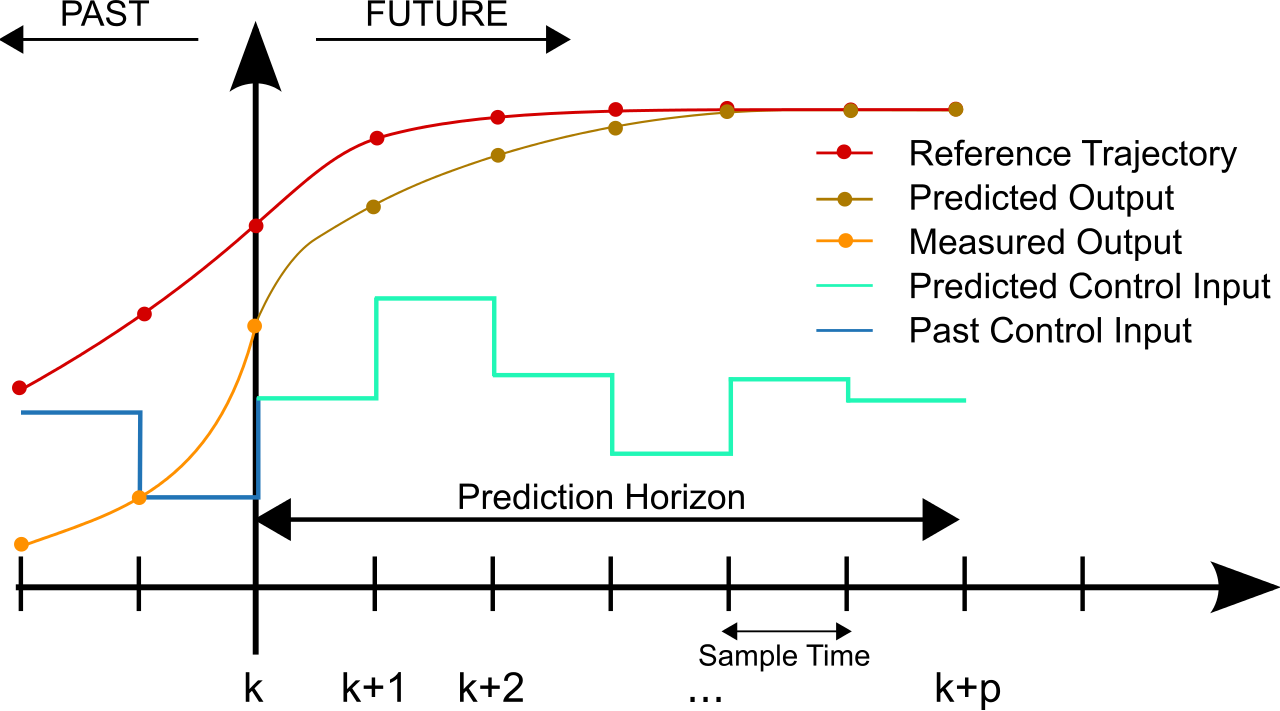
\includegraphics[width=0.5\textwidth]{MPC_scheme}
		\caption{A simple MPC diagram from the wikipedia page \cite{Wikipedia}}
		\label{fig:MPC diagram}
	\end{figure}
			
	\subsection{System}
		
	\subsection{Problem definition}
		\subsubsection{Problem form}
			The goal is to define the problem as equation~\ref{eq:PANOC MPC form}, and then solve it for u given $x_0$, the current state of the system. Sometimes $x_0$ will be assumed to be part of the function f, just like the reference state and input. Which leads to the simplified equation, equation~\ref{eq:PANOC form} .
			\begin{equation}
				\underset{u}{\minimize} \  f(x_0,u) + g(u)
				\label{eq:PANOC MPC form}
			\end{equation}
			
			\begin{equation}
				\underset{u}{\minimize} \  f(u) + g(u)
				\label{eq:PANOC form}
			\end{equation}
		\subsubsection{Direct Single shoot}
			If the horizon is N then the problem is solved for the inputs $u=[u_0,u_1,... u_{N-1}]$ where each $u_k$ is a vector of all the inputs of the system. This means that the vector u is of size Horizon $\cdot$ dimension\_input .
			
			The cost for each step in the horizon is defined as \ref{eq:single shot iteration cost}, this is called the stage cost.
			\begin{equation}
				\begin{aligned}
				& l_k(x_0,u) = &&  x_k^T Q x_k  +  u_k^T R u_k \\
				& \text{subject to}			&& x_0 = \bar{x} \\
				& 							&&  x_{n+1} = F_d(x_n,u_n), n=0...N-1
				\end{aligned}
				\label{eq:single shot iteration cost}
			\end{equation}
			
			The terminal cost is a special case of the stage cost as it is the last stage cost in the horizon. So if the Horizon=N the terminal cost can defined as equation~\ref{eq:single shot terminal cost}.
			
			\begin{equation}
				\begin{aligned}
					& l_N(x_0,u) = && x_N^TSx_N \\
					& \text{subject to}			&& x_0 = \bar{x} \\
					& 							&&  x_{n+1} = F_d(x_n,u_n), n=0...N-1
				\end{aligned}
				\label{eq:single shot terminal cost}
			\end{equation}
			
			$f(x_0,u)$ can then be defined as in equation~\ref{eq:single shot definition}, the sum of the stage costs and the terminal cost.
			\begin{equation}
				f(x_0,u) = \sum_{k=1}^{N-1} l_k(x_0,u) + l_N
				\label{eq:single shot definition}
			\end{equation}
			
			As a side note, an other term can be added to equation~\ref{eq:single shot definition} to represent the obstacle avoidance. More on this later on in this chapter in the subsection on obstacles.
		\subsection{Direct Multiple shoot}
			The multiple shoot needs more information than just an initial state. It requires an initial estimate of all of the intermediate states. The state estimates will be referred to as $x_i$ and the states derived from the estimate and its corresponding input will be referred to as $\bar{x_i}$. As before the goal of the optimization algorithm is to find the optimal inputs $u_i$, so that the cost function is as low as possible. And additionally  $\bar{x_i} - x_{i+1} = 0$, called the continuity conditions.
			
			\begin{equation}
				\bar{x_i} = F(x_i,u_i)
				\label{eq:}
			\end{equation}
			
			The continuity conditions are displayed in equation~\ref{eq:continuety condition multiple shot} and were not necessary in single shot as there are no state estimates like $\bar{x}$. If when starting the algorithm the initial state estimates are relatively close to the solution, a significant speed increase can be accomplished. As information was incorporate into the algorithm.
			
			\begin{equation}
				\bar{x_i} - x_{i+1} = 0
				\label{eq:continuety condition multiple shot}
			\end{equation}
			
			The direct multiple shoot definition looks like equation~\ref{eq:multiple shot cost} and has an extra equality condition compared to the single shoot. This equality condition will be added as a soft constraints to the cost function. This is displayed in equation~\ref{eq:multiple shot cost with soft constraint} and will be used in the practical implementation.
			
			\begin{equation}
				\begin{aligned}
				L =  & \sum_{i=1}^{N} l(\bar{x_i},u_i) \\
				& \text{subject to}			&& \bar{x_i} = F(x_i,u_i) \\
				& 							&& \bar{x_i} - x_{i+1} = 0
				\end{aligned}
				\label{eq:multiple shot cost}
			\end{equation}
			
			\begin{equation}
			\begin{aligned}
			L =  & \sum_{i=1}^{N} l(\bar{x_i},u) + ||\bar{x_i} - x_{i+1}||\\
			& \text{subject to}			&& \bar{x_i} = F(x_i,u_i) \\
			\end{aligned}
			\label{eq:multiple shot cost with soft constraint}
			\end{equation}
			
		\subsection{Obstacle avoidance}
			The obstacle avoidance is based on the soft constraint definition described in \cite{AjaySathya2017}. It can be described as a set or an constraint.
			\subsubsection{As set}
				An obstacle can be defined as an open set, as illustrated by equation~\ref{eq:obstacle as open set}. It is defined by the intersection of a set of nonlinear inequalities.
				\begin{equation}
					O = {z \in \Re^d : h^i(z)>0,\ i \in N}
					\label{eq:obstacle as open set}
				\end{equation}
				
			\subsubsection{As constraint}
				\begin{equation}
					[z]_+ =  \max\{0,z\}
				\end{equation}
				
				The statement $h(x)<0$ is equivalent to saying $[h(x)]_+=0$, so equation~\ref{eq:obstacle as open set} is equivalent to setting equation~\ref{eq:obstacle as equality} to zero.
				
				\begin{equation}
					\Phi_0(z) =  \frac{1}{2} \prod_{i=1}^m \Big( [h^i(z)]_+ \Big)^2
					\label{eq:obstacle as equality}
				\end{equation}
				
				The gradient of equation~\ref{eq:obstacle as equality} is define as equation~\ref{eq:obstacle as equality}
				
				\begin{equation}
					\nabla \Phi =
					\begin{cases}
						\sum_{i=1}^{m} h^i(z)\prod_{j \ne i} \Big( [h^i(z)]_+ \Big)^2 \nabla h^i(z)
						& x \in O \\
						0 & else
					\end{cases}
					\label{eq:derivative obstacle as equality}
				\end{equation}
			
			\subsubsection{Polyhedral obstacle}
				A simple obstacle example of such an obstacle is a polyhedral as defined in equation~\ref{eq:polyhedral constraint}.
				\begin{equation}
					\prod \Big([b_i - a_i^t z]_+ \Big)^2 = 0
					\label{eq:polyhedral constraint}
				\end{equation}
			
			\subsubsection{Obstacle as soft constraint}
				The obstacle avoidance is added as a soft constraint to the cost function. As demonstrated in equation~\ref{eq:derivative obstacle as equality}, this definition is two times differentiable and so this does not break the condition that the cost functions needs a gradient to be solved with the PANOC algorithm.
			
		\subsection{Input constraints}
			An other important aspect of a MPC problem are input constraints. In practice inputs have to comply with the physical properties of the devices. Absurdly high or low input values might in theory lead to a fast solution, but are not feasible in practice.
			
			A major advantage of the PANOC algorithm is that it can take non linear or non convex constraints. As longs as the proximal operation is analytically defined on the constraint it is feasible. 
			
			A simple example is the indicator box function, which allows to set a maximum and minimum value on the inputs. (The indicator box function is defined in the appendix) The indicator box function as input constraint can demand that every feasible solution lies within the bounds of the user defined box.
\chapter{Proximal gradient method}
	\subsection{Proximal mapping}
		The proximal operator is defined as $\prox_g(x)= \underset{u}{\argmin}(g(u) + \frac{1}{2 \gamma}||u-x||^2_2)$. 
		
		\begin{itemize}
			\item if $h(x)=0$ then $\prox_h(x)=x$ 
			\item if $h(x)=I_c(x)$ where $I_c$ is define in \eqref{eq:indicator function}, the proximity operator on an indicator function is the orthogonal projection on the set.
		\end{itemize}
		
		The indicator function: is defined in equation ~\eqref{eq:indicator function}.
		\begin{equation}
			I_c = 
			\begin{cases}
			0 & x \in C  \\
			\infty & x \notin C
			\end{cases}
			\label{eq:indicator function}
		\end{equation}
		
		The proximal mapping can be seen as a generalization of a projection. The Appendix contains an other important example, the indicator box function.
	
	\subsection{Gradient projected method}
		
		\begin{equation}
			\begin{aligned}
			& \underset{x}{\text{argmin}}
			& & f_0(x) \\
			& \text{subject to}
			& & g(x)=0
			\end{aligned}
			\label{eq:prox grad opti problem}
		\end{equation}
		
		The classical gradient decent method cannot be used to solve the problem of \eqref{eq:prox grad opti problem}. As this problem has a condition that must be met by the algorithms solution. If in each iteration the solution is projected on the space spanned by $g(x)=0$ the iteration \eqref{eq:grad descent} becomes \eqref{eq:projected grad descent}. This algorithm is called the gradient projection method.
		
		\begin{equation}
			x^k = x^{k-1} - \gamma \nabla f(x^{k-1})
			\label{eq:grad descent}
		\end{equation}
		
		\begin{equation}
			x^k = \project_{g(x)=0}[ x^{k-1} - \gamma \nabla f(x^{k-1})]
			\label{eq:projected grad descent}
		\end{equation}
		
		If $g(x)$ is the indicator function of the set onto which is projected. Then  \eqref{eq:projected grad descent} can be written as \eqref{eq:proximal grad descent}, known as the proximal gradient method.
		
		\begin{equation}
				x^k = \prox_{\gamma g}[ x^{k-1} - \gamma \nabla f(x^{k-1})]
			\label{eq:proximal grad descent}
		\end{equation}
	
	\subsection{The proximal gradient method}
		\eqref{eq:prox grad problem} Can be solved with the proximal gradient method, sometimes called forward backward splitting - FBS . Where the proximal mapping of $g(x)$ is analytically defined. 
			\begin{equation}
			\underset{x}{\argmin} = f(x) + g(x)
			\label{eq:prox grad problem}
			\end{equation}
		
		Inspired by the projected gradient method, the proximal gradient method is defined as \eqref{eq:prox grad method}. The $\gamma$ variable is the step size, in order to have a convergence of O(1/k) $\gamma \in(0,1/L)$. If $\gamma \in (1/L,2/L)$ the algorithm will still converge but then its no longer a majorization-minimization method. (more on this see \cite{NealParikh})
		
		\begin{equation}
			x^k = \prox_{\gamma g}\big( x^{(k-1)}- \gamma \nabla f(x^{(k-1)})\big)
			\label{eq:prox grad method}
		\end{equation}	
	
	\subsection{Proximal minimization algorithm}
		 \cite{QianYang} Contains a short proof that illustrates the proximal mapping as a fixed point minimization algorithm. A property of the conjugated function is used to derive the gradient, see appendix for the theorem.
		 \begin{proof}
		 	the iteration $x^{k+1}=\prox_g(x^k)$ will minimize the smoothed version of function f(x) 
		 	\begin{align*}
		 	f_{\mu}
		 	&= \underset{y}{\inf}\Big\{ |y| +\frac{1}{2 \mu}(x-y)^2 \Big\} \\
		 	&=   \frac{1}{2 \mu}||x||^2 + \frac{1}{2\mu} 
		 	\underset{y}{\inf}\Big\{
		 	2 \mu f(y) - 2x^T y + ||y||^2
		 	\Big\} \\
		 	&=  \frac{1}{2 \mu}||x||^2 + \frac{1}{\mu} 
		 	\underset{y}{\sup}\Big\{
		 	x^T y  - \mu f(y) - \frac{1}{2} ||y||^2 \Big \} \\
		 	&= \frac{1}{2\mu }||x||^2 \frac{1}{\mu } \Big( \mu f + \frac{1}{2}||\cdot||^2 \Big)^* (x) \\
		 	\nabla  f_{\mu} 
		 	&= \frac{x}{\mu} - \frac{1}{\mu} \underset{y}{\argmax} 
		 	\Big \{ x^Ty - \mu f(y) - \frac{1}{2}||y||^2 \Big \}\\
		 	& = \frac{1}{\mu}(x - \prox_{\mu f}(x)) \\
		 	\prox_{\mu f}(x)
		 	& = x- \mu \nabla f_{\mu}(x)
		 	\end{align*}
		 	\label{prf:proximal minimiztion alg proof}
		 \end{proof}

		 This means thats the iteration $x^{k+1}=\prox_g(x^k)$ will minimize the smoothed version of function g(x). 

\section{Proximal gradient method with line search}
	\subsection{Starting value gamma }
		\subsubsection{Estimating Lipschitz value}
			The Lipschitz of $\nabla f(x)$ value is a non negative number that complies with \eqref{eq:definition lipschitz value}.
			\begin{equation}
			L = \underset{x \neq y}{\sup} \frac{|\nabla f(y)-\nabla f(x)|}{|y-x|}
			\label{eq:definition lipschitz value}
			\end{equation}
			
			In practice it is not always possible to find the actual Lipschitz value. So the Lipschitz value is estimated ($L'$) locally at the starting location $x_0$ of the algorithm using \eqref{eq:estimated lipschitz value in starting position}. With $\delta=max[\delta_l,10^{-6} \cdot x_0]$ where $\delta_l$ is a small number chosen by the controller designer.
			% in code the safety value is DELTA_LIPSCHITZ_SAFETY_VALUE and set to 10^-6
			
			\begin{equation}
			L' = \frac{|\nabla f(x_0+\delta)-\nabla f(x_0)|}{|\delta|}
			\label{eq:estimated lipschitz value in starting position}
			\end{equation}
			
			The Lipschitz value is not explicitly saved but is used to estimate the line-search parameter $\gamma$. The backtracking of the proximal gradient descent then further improves this estimate. As the algorithm progresses and $\gamma$ improves, so does the estimation of the Lipschitz value indirectly.
		
		\subsubsection{Estimating gamma}	
			From \cite{LorenzoStella2017} it is known that $\gamma<\frac{1}{L}$ in order to guarantee convergence to a local minimum. As gamma needs to be smaller than $\frac{1}{L}$ a safety value is introduced. This idea was copied over from the kul-forbes/ForBES library by Lorenzo Stella and Panos Patrinos, which uses a $\beta$ of 0.05. And leads to \eqref{eq:starting value gamma}.
			\begin{equation}
			\gamma = \frac{1-\beta}{L}
			\label{eq:starting value gamma}
			\end{equation}		
	
	\subsection{Backtracking gamma}
		\subsubsection{Backtracking algorithm}
			Line-search is based on "Armijo's sufficient decrease condition" written down as \eqref{eq:Armijo's sufficient decrease condition}. The safety parameter $\theta$ multiplied with the step size $t_k$ is $\gamma=\theta \cdot t_k$. 
			
			\begin{equation}
			f(x_k + t_kp_k) \leq f(x_k) + \theta t_k \nabla f(x_k)^Tp_k
			\label{eq:Armijo's sufficient decrease condition}
			\end{equation}
			
			Line-search more specific backtracking will reduce the value of $\gamma$ until the condition of \eqref{eq:Armijo's sufficient decrease condition} fails.
			
		\subsubsection{Backtracking in proximal gradient descent used in FBS}
			The  "Armijo's sufficient decrease condition" is adjusted to \eqref{eq:Armijo's sufficient decrease condition prox grad PANOC} Which is an quadratic bound, $-p_k=x-\bar{x}$ and an additional term $\frac{1-\beta}{2 \gamma}||x-\bar{x}||^2$ is added.
			
			\begin{equation}
			f({\bar{x}}) \leq f(x) - \nabla f(x)^T[x-\bar{x}] + \frac{1}{2 \gamma}||x-\bar{x}||^2
			\label{eq:Armijo's sufficient decrease condition prox grad PANOC}
			\end{equation}
			
			This all leads to algorithm~\ref{alg:backtracking on gamma} the proximal gradient method. \eqref{eq:Armijo's sufficient decrease condition prox grad PANOC} can be seen as a quadratic model, as the Lipschitz value of the gradient is equal to $L=\frac{1}{\gamma}$.
			
			\begin{algorithm}
				\caption{backtracking $\gamma$}
				\label{alg:backtracking on gamma}
				\begin{algorithmic}[1]
					\Procedure {lineasearch\_gamma}{x,$\gamma$}
					\State $\bar{x} = \prox_{\gamma g}\big( x- \gamma \nabla f(x)\big)$
					\While{$f({\bar{x}}) > f(x) - \nabla f(x)^T[x-\bar{x}] + \frac{1}{2 \gamma}||x-\bar{x}||^2$}
					\State $\gamma = \frac{\gamma}{2}$
					\State $\bar{x} = \prox_{\gamma g}\big( x- \gamma \nabla f(x)\big)$
					\EndWhile
					\State \Return $\gamma$
					\EndProcedure
				\end{algorithmic}
			\end{algorithm}
	\subsection{Final algorthm}
		The final algorithm~\ref{alg:proximal gradient PANOC with backtracking} delivers the upward direction. $x_{k+1}=x_k - direction$.
		\begin{algorithm}
			\caption{proximal gradient PANOC with backtracking}
			\label{alg:proximal gradient PANOC with backtracking}
			\begin{algorithmic}[1]
				\Procedure{get\_proximal\_gradient\_step}{x,$\gamma$}
				\State $\gamma$=LINESEARCH\_GAMMA($\gamma$)
				\State $\bar{x} = \prox_{\gamma g}\big( x- \gamma \nabla f(x)\big)$
				\State \Return direction=$[x-\bar{x}]$, $\gamma$
				\EndProcedure
			\end{algorithmic}
		\end{algorithm}
\section{Proximal gradient alternative view}
	\subsection{Majorization-minimization algorithm}
	A Majorization-minimization algorithm, is a type of algorithm that minimizes a surrogate function. The surrogate function is a approximation of the actual problem. And needs to have the conditions described in \eqref{eq:MM algorithm conditions}, where h(x,y) is a surrogate function and f(x) is the actual problem. The problem described in \eqref{eq:MM algorithm formula step} is iteratively solved until convergence.
	\begin{equation}
		\begin{cases}
			h(x,x) = f(x) \\
			h(x,y) \leq f(x)
		\end{cases}
		\label{eq:MM algorithm conditions}
	\end{equation}
	
	\begin{equation}
		x_{k+1} = \argmin_y h(x_k,y)
		\label{eq:MM algorithm formula step}
	\end{equation}

	\subsection{The proximal gradient as majorization-minimization algorithm}
	The proximal gradient algorithm can be seen as a majorization-minimization algorithm. Its surrogate function is described in \eqref{eq:surrogate function}, proof~\ref{prf:proximal gradient as MM} illustrates how minimizing the surrogates function is equal as taking a step of the proximal gradient algorithm.
	
	\begin{equation}
		h(x,y) = f(x) + \nabla f(x)^T(x-y) + \frac{1}{2 \cdot \gamma}||x-y||^2_2
		\label{eq:surrogate function}
	\end{equation}
	
	\begin{proof}
		$h(x,y) = f(x) + \nabla f(x)^T(x-y) + \frac{1}{2 \cdot \gamma}||x-y||^2_2$ is the MM surugate function of proximal gradient algorithm. The gradient is set too zero and solved for y.
		\begin{align*}
		h(x,y)
		& = f(x) + \nabla f(x)^T(x-y) + \frac{1}{2 \cdot \gamma}||x-y||^2_2 \\
		\frac{\partial h(x,y)}{\partial y}
		& = 0 + \nabla f(x) + \frac{1}{2 \cdot \gamma} + \frac{1}{2 \cdot \gamma}\frac{\partial ||x-y||^2_2}{\partial y}  \\	
		\frac{\partial ||x-y||^2_2}{\partial y}
		& = \frac{\partial(x-y)^T(x-y)}{\partial y} = \frac{\partial(-2x^Ty + y^Ty)}{\partial y} = -2x+y \\
		\frac{\partial h(x,y)}{\partial y}
		& = \nabla f(x) - \frac{x}{\gamma} + \frac{y}{2 \gamma} = 0 \\
		0
		& = \gamma \nabla f(x) - x + \frac{y}{2} \\
		y & = \gamma \nabla f(x) - x
		\end{align*}
		\label{prf:proximal gradient as MM}
	\end{proof}
\chapter{PANOC algorithm}
	This section is based on \cite{LorenzoStella2017} and \cite{AjaySathya2017}, the difference is that this text is focused implementation. And so the formula's often look slightly different. The Forward backward envelop part is based on \cite{Themelis}, which contains a slightly different algorithm that also uses the Forward backward envelop.
	\section{Introducing panoc}
		The PANOC algorithm is an accelerated version of the proximal gradient descent. The direction  $x-\bar{x}$ is a combination of the proximal gradient algorithm and second direction that makes use of curvature information. This second direction will hopefully accelerate the convergence of the algorithm.
		
		\begin{equation}
		x_{k+1} = x_k + (1-\tau_k)\cdot (x-\bar{x}) + \tau_k d_k
		\end{equation}
		
		The new term $\tau_kd_k$ should accelerate the convergence if $\tau_k\neq0$. The step $d_k$ is calculated using a quasi-newton algorithm. As a quasi-newton algorithm uses curvature information of the cost function, it uses information not available to a gradient descent based method. 
		
		Furthermore it has a super linear convergence rate when it gets close to the solution. Which is much faster then the sub-linear convergence of a gradient descent algorithm . On top of that, the quasi-newton method will not require extra function evaluations. Which are the major contributors to the costs of the algorithm.
		
	\section{Quasi newton method}
		\subsubsection{Problem definition}
			The iteration of equation~\ref{eq:prox grad method} can indirectly be used to solve the optimization problem.  By using the residue defined in equation~\ref{eq:residue prox grad method} a fixed point can be found. 
			
			\begin{equation}
			R_{\gamma}(x)= \frac{1}{\gamma}\left[ x - \prox_g( x - \nabla f(x)\gamma) \right]
			\label{eq:residue prox grad method}
			\end{equation}
			
			The solution of equation~\ref{eq:residue prox grad method} can be found trough the Newton iteration of equation~\ref{eq:newton iteration residual}. Where $H_k$ satisfies the inverse secant condition of equation~\ref{eq:newton iteration residual inverse secant}. As the implementation is aimed at embedded software a good option to solve this would be L-BFGS. More on this in the chapter on L-BFGS.
			
			\begin{equation}
			x^{k+1} = x^k -H_kR_{\gamma}(x^k)
			\label{eq:newton iteration residual}
			\end{equation}
			\begin{equation}
			x^{k+1} - x^k = H_{K+1} \Big( R_{\gamma}(x^{k+1})- R_{\gamma}(x^k) \Big)
			\label{eq:newton iteration residual inverse secant}
			\end{equation}
		
	\section{Forward backward envelop}	
		Newton iterations only converge quickly when they are close to the solution. In order to get better global behavior a proper global strategy is required. The optimization problem is changed from $\varphi(x) = f(x) + g(x)$ to equation~\ref{eq:FBE definition using Moreau envelope}. This problem is smoother while it still has the same optimal solution.(proof see \cite{LorenzoStella2017} and \cite{Themelis}) The same $\gamma$ as with the proximal gradient should be used, notice how the FBE contains the line-search condition use in the proximal gradient. (more on the FBE in \cite{Themelis})
		
		The Moreau envelope is de define as \ref{eq:Moreau envelope}, this smooths the function, and has a close relationship with the proximal operator as illustrated earlier. Using simple algebra equation~\ref{eq:FBE definition using Moreau envelope} can be transformed into equation~\ref{eq:FBE definition using quadratic approximation}.(proof in Appendix) The solution $y$ of the infimum defined in equation~\ref{eq:FBE definition using quadratic approximation} is $\bar{x}$. Considering the close relationship between the Moreau envelope and the proximal operator (see more in \cite{Themelis}) this is to be expected.
		
		An alternative way to look the FBE is illustrated in \cite{AjaySathya2017}, where the problem can be seen as minimizing a quadratic approximation  $f(x) +  \nabla f(x)^T(y-x) + g(y) + \frac{1}{2 \gamma} ||x-y||^2  $ towards y in point x.  Remember that $L = \frac{1}{\gamma}$, with L being the Lipschitz constant of the gradient.
		
		\begin{equation}
			g^{\gamma} = \underset{y}{\inf} \big \{f(y)+\frac{1}{2 \cdot \gamma}||x-y||^2 \big \}
			\label{eq:Moreau envelope}
		\end{equation}
		
		\begin{equation}
		\varphi_{\gamma} = f(x) - \frac{\gamma}{2}||\nabla f(x)||^2 + g^{\gamma} \big(x-\gamma \nabla f(x) \big)
		\label{eq:FBE definition using Moreau envelope}
		\end{equation}
		
		\begin{equation}
		\varphi_{\gamma} =   f(x) + \underset{y}{\inf} \Big\{ \nabla f(x)^T(y-x) + g(y) + \frac{1}{2 \gamma} ||x-y||^2  \Big\}
		\label{eq:FBE definition using quadratic approximation}
		\end{equation}
		
		\begin{proof}
			The solution to the infimum of equation~\ref{eq:FBE definition using quadratic approximation} is y=$\bar{x}= \prox_g(x-\gamma \nabla f(x))$
			\begin{align*}
			\prox_g(\bar{x}) 
			&=\prox_g(x- \gamma \nabla f(x)) \\
			&= \underset{y}{\argmin} \Big \{ g(y) 
			+ \frac{1}{2 \gamma}||(y-x) + \gamma \nabla f(x)||^2 \Big \} \\
			&= \underset{y}{\argmin} \Big \{ g(y) 
			+ \frac{1}{2 \gamma} \big[||y-x||^2 + 2 \gamma \nabla f(x)^T(y-x) + ||\nabla f(x)||^2\gamma^2 \big] \Big \} \\
			&= \underset{y}{\argmin} \Big \{ g(y) 
			+ \frac{1}{2 \gamma} \big[||y-x||^2 + 2 \gamma \nabla f(x)^T(y-x)  \big] \Big \}\\
			&= \underset{y}{\argmin} \Big \{   \nabla f(x)^T(y-x)  + g(y) 
			+ \frac{1}{2 \gamma} ||y-x||^2  \Big  \}
			\end{align*}
			\label{prf:prox is solution to FBE inf}
		\end{proof}
		
		Equation~\ref{eq:practical implementation of FBE} is the practical implementation of the FBE. The parameter gamma is the line-search parameter used in the proximal gradient descent. The first 3 terms are the same as with the line-search on $\gamma$, the last term $g(\bar{x})$ is new and makes sure the solution complies with the constraint.
		
%		\cite{AjaySathya2017} has an excellent example to illustrate this.(figure~\ref{fig:FBE illustration}).
%		
		\begin{equation}
			\begin{aligned}	
				& \varphi(\gamma,x)= 
				&& f(x) - \nabla f(x)^T(x-\bar{x}) + \frac{1}{2 \gamma}||x-\bar{x}||^2  + g(\bar{x})
				\\
				& with 
				&&\bar{x} = \prox_g( x - \gamma\nabla f(x)) 
			\end{aligned} 
			\label{eq:practical implementation of FBE}
		\end{equation}
		
%		\begin{figure}[H]
%			\centering
%			\label{fig:FBE illustration}
%			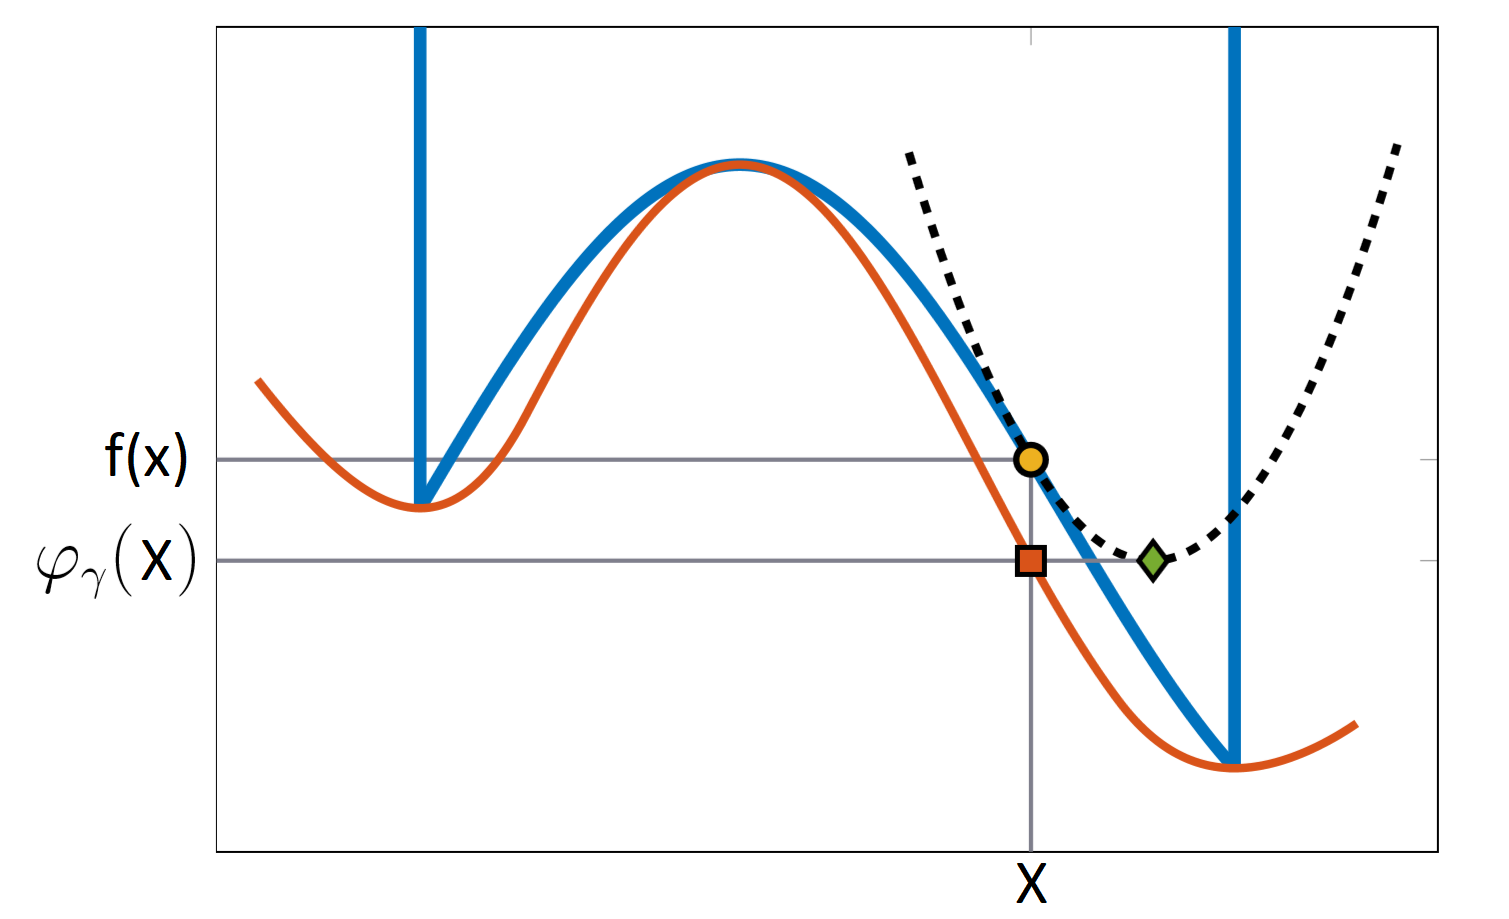
\includegraphics[width=0.6\textwidth]{FBE}
%			\caption{FBE example copied over from \cite{AjaySathya2017}, red is?? blue is ?? TODO expain this figure}
%		\end{figure}
	
	\section{Line-search with FBE}
	In \cite{LorenzoStella2017} the line-search condition is specified as equation ~\ref{eq:line-search with FBE}. The line-search parameter $\tau$ determines $x^{k+1}$ by choosing the convex combination of the step from the proximal gradient and the L-BGFS as defined in equation~\ref{eq:linea-search tau definition}.  \cite{LorenzoStella2017} specifies that $\sigma \in (0, \gamma \frac{1-\gamma\cdot L}{2})$. As stated before it is assumed that $L=\frac{1-\beta}{\gamma}$, some simple algebra will lead to the condition $\sigma \in (0,\frac{\beta \gamma}{2})$.
	
	 Equation~\ref{eq:practical line-search with FBE} is the practical implementation of equation~\ref{eq:line-search with FBE}. A new constant $\alpha \in (0,1)$ is introduced, an possible value for $\alpha$ would be 0.5 ($\alpha=0.5$ is the choice used by the Matlab implementation of PANOC in ForBes known as zerofpr2).
	
	\begin{equation}
		x^{k+1} = u_k - (1-\tau_k)\cdot (x-\bar{x}) + \tau \cdot dir_{LBFGS}
		\label{eq:linea-search tau definition}
	\end{equation}
	
	\begin{eqnarray}
		\label{eq:line-search with FBE}
		\varphi_{\gamma}(x^{k+1})\leq\varphi_{\gamma}(x^{k}) - \sigma ||\frac{x-\bar{x}}{\gamma}||^2 \\
		=
		\varphi_{\gamma}(x^{k}) - \frac{\sigma}{\gamma^2} ||x-\bar{x}||^2
	\end{eqnarray}
	
	\begin{equation}
		\varphi_{\gamma}(x^{k+1}) \leq 		\varphi_{\gamma}(x^{k}) - \alpha \frac{\beta }{\gamma \cdot 2} ||x-\bar{x}||^2
		\label{eq:practical line-search with FBE}
	\end{equation}
	
	
		
		\begin{algorithm}
			\caption{PANOC}
			\label{alg:PANOC}
			\begin{algorithmic}[1]
				\Procedure {PANOC\_GET\_NEW\_LOCATION}{$x^k$,$\gamma$}
				\State [$(x-\bar{x})$ , $\gamma$] = GET\_PROXIMAL\_GRADIENT\_STEP($\gamma$,$x^k$)
				\State $ dir_{LBFGS}$ = LBFGS($x^k$)
				\State $\tau =1$
				\State $x^{k+1} = x_k - (1-\tau_k)\cdot (x-\bar{x}) + \tau \cdot dir_{LBFGS}$
				\While{$\varphi_{\gamma}(x^{k+1}) > 		\varphi_{\gamma}(x^{k}) - \alpha \frac{\beta}{\gamma \cdot 2} ||(x-\bar{x})||^2$}
				\State $\tau = \tau / 2$
				\State $x^{k+1} = x_k - (1-\tau_k)\cdot (x-\bar{x}) + \tau \cdot dir_{LBFGS}$
				\EndWhile
				\EndProcedure
			\end{algorithmic}
		\end{algorithm}
	
%\chapter{Conclusion}
\label{cha:conclusion}

\section{Nmpc-codegen library}
The controller code generation and simulation is available in both Python and Matlab, which are computer languages with a fast learning curve. It is very straightforward for a control engineer to design and test a controller, without knowing anything about low level programming.

The generated controller, has a simple interface that requires nearly no control theory knowledge. So that the user of the generated C library doesn't necessarily has to be a control engineer but could be an embedded software engineer. Who has no idea how a MPC controller works, but knows how embedded systems work.

However as the MPC problem becomes more complex. The algorithm can get stuck on a local minimums, which might not be a viable solution. It might violate the constraint by a too large margin. This can partially be avoided by properly tuning the weights of the constraints. 

This weight tuning is rather hard, as increasing the weights worsens the condition of the problem. So the controller designer often ends up with an impossible choice. The last chapter partially solves this by using a Lagrangian. It is easier to tune the parameters and it improves the performance of the controller. 

\section{Future work}
The PANOC algorithm does not require advanced algebra operations such as solving a system. Only simple vector additions and inner product are required. So it's straightforward to implement PANOC with flip-flops and adders. The only hard part is the cost function and it's gradient, as Casadi does not support VHDL or Verilog at this time.

\section{Industrial applications}
Embedded model predictive control is used in a wide variety of domains, here are a few examples:
\begin{itemize}
	\item Unmanned Aerial vehicles (UAV's)
	\item Self driving robots
	\item Anti-lock brakes cars
	\item Adaptive cruise control cars
	\item Robotics
\end{itemize}

%%% Local Variables: 
%%% mode: latex
%%% TeX-master: "thesis"
%%% End: 

% If you have appendices:
%\appendixpage*          % if wanted
%\appendix
%\chapter{The First Appendix}


%%% Local Variables: 
%%% mode: latex
%%% TeX-master: "thesis"
%%% End: 



\backmatter
% The bibliography comes after the appendices.
% You can replace the standard "abbrv" bibliography style by another one.
\bibliographystyle{abbrv}
\bibliography{references}

\end{document}